%%%%%%%%%%%%%%%%%%%%%%%%%%%%%%%%%%%%% BEGIN HEADERS %%%%%%%%%%%%%%%%%%%%%%%%%%%%%%%%%%%%%%%%%%%%%%%%%%%%%
\documentclass[11pt,conference]{IEEEtran}

\usepackage{longtable}
\usepackage{graphicx}
\usepackage[utf8]{inputenc}
\usepackage{fancyhdr}
\usepackage{float}
\usepackage[hidelinks]{hyperref}
\usepackage{listings}
\usepackage{color}
\usepackage{natbib}
\usepackage{caption}

% Your names in the header
\pagestyle{fancy}
\rhead{Enrico Tedeschi, Mike Murphy}
\lhead{INF-3200 Distributed Systems - Assignment 2}
\cfoot{\thepage}

% Used for including code in a stylized manner
\definecolor{codegreen}{rgb}{0,0.6,0}
\definecolor{codegray}{rgb}{0.5,0.5,0.5}
\definecolor{codepurple}{rgb}{0.58,0,0.82}
\definecolor{backcolour}{rgb}{0.95,0.95,0.92}
 

\lstdefinestyle{mystyle}{
    backgroundcolor=\color{backcolour},   
    commentstyle=\color{codegreen},
    keywordstyle=\color{magenta},
    numberstyle=\tiny\color{codegray},
    stringstyle=\color{codepurple},
    basicstyle=\footnotesize,
    breakatwhitespace=false,         
    breaklines=true,                 
    captionpos=b,                    
    keepspaces=true,                 
    numbers=left,                    
    numbersep=5pt,                  
    showspaces=false,                
    showstringspaces=false,
    showtabs=false,                  
    tabsize=2
}

\lstset{style=mystyle}

% The Title
\title{UiT INF-3200 Distributed Systems - Project 2\\Fall 2015}

% Your name and email
\author{Enrico Tedeschi\\ete011@post.uit.no
    \and Mike Murphy\\mmu019@post.uit.no}


%%%%%%%%%%%%%%%%%%%%%%%%%%%%%%%%%%%%% END HEADERS %%%%%%%%%%%%%%%%%%%%%%%%%%%%%%%%%%%%%%%%%%%%%%%%%%%%%

\begin{document}

% Create the title and everything
\maketitle


\section{Introduction}

Our task was to implement leader election on top of a peer-to-peer network.

All the peers in the network must agree on who the leader is and only one peer can be leader at a time. Provides support for peers joining and leaving the network.


\subsection{Requirements}

\begin{itemize}
\item Support at least 10 nodes in a p2p network structure of your own choice. No centralized architectures allowed; i.e. all processes should behave similarly.
\item Support graceful shutdown of nodes. On receiving a signal to shut down(SIGTERM), a node should leave the network.
\item Support adding nodes on demand. Adding a new process allows you to grow the system as the demand increases.
\item Leader election. There should at all times be a single leader. A pertinent Q: What happens if the leader leaves the network?
\item A GET request to any node for the url "/getCurrentLeader" should return the ip and port of the current leader. The response body must be formatted as a single ip:port (e.g. "127.0.0.1:1234") entry.
\item A GET request to any node for the url "/getNodes" should return a list of ip and port pairs of all nodes connected to the recipent node. The response body must be formatted as a list of ip:port (e.g. "127.0.0.1:1234") entries with newline separating each ip:port pair.
\item Measure the time it takes to elect a leader when the number of nodes changes.
\end{itemize}


\section{Technical Background}
To solve the problem some technical background are required. First of all, a good knowledge about programming and some basic concept about distributed systems is necessary. Is good to know and to study then, some of the possible election algorithms which could be used. We took into consideration the \textit{Bully algorithm} and the \textit{Ring algorithm election}.

\subsection{Bully algorithm}
When a new leader is needed a process \textit{P} send an election message to all the nodes with an higher ID number. If there are no answers, \textit{P} wins the election. If \textit{P} gets an answer then it terminates his job and the election continues with the node with the higher value just called. In the Fig \ref{fig:bully} the node 3 starts the election because the previous leader 6 crashed. The new leader will be the node 5.
\begin{figure}[h!]
  \centering
    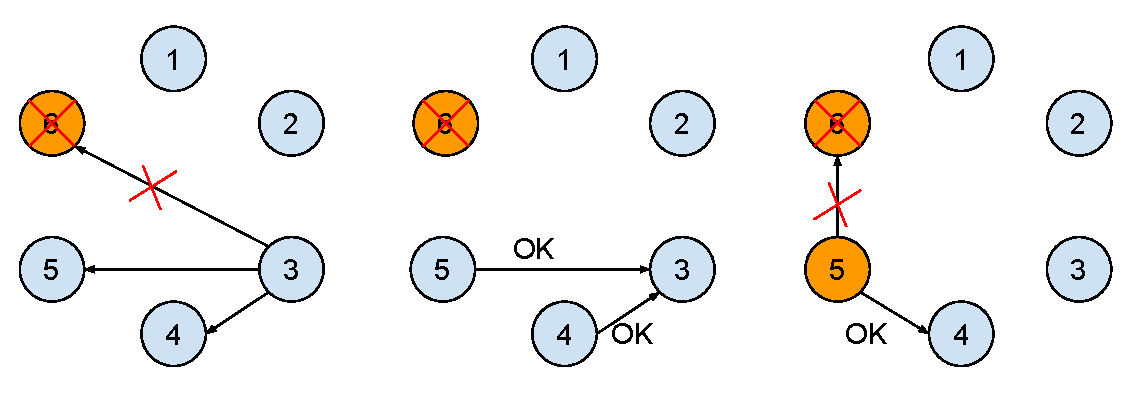
\includegraphics[width=0.5\textwidth]{bully}
    \caption{Example of how the bully algorithm works, the leader changes from 6 to 5}
    \label{fig:bully}
\end{figure}

\subsection{Ring algorithm election}
%TODO: describe the ring algorithm and put an illustration

%TODO: talk about leader, algorithm election, and problems in joining and leaving

\section{Design}

%TODO: talk about the ring design and which one was chosen in the implementation

\section{Implementation}

%TODO: talk about why the ring algorithm was chosen (because from the previous version of the implemented network each node has information about his successor -- which is required for the ring algorithm)

\subsection{Languages and Code}

Our solution is implemented in a mix of Python and Bash script, Python for the
actual node implementation, and a Bash script to communicate through the network created, adding and removing nodes.

We started with skeleton code by our first assignment for what concerns the node and the script code. 
The code was rearranged by removing the front-end node and by adding some properties to the nodes such as the predecessor node and information about the leader, which at the beginning, is the first node joining the network.

The code were tested before on local machine, using bash scripts and the given visual test code from Einar Holsbø Jakobsen and Magnus Stenhaug and then on the uvrocks cluster.

\subsection{Network Protocol}

The backend nodes accept and retrieve data through a simple HTTP API. HTTP's PUT
and GET operations are a natural fit for a key-value store, as their semantics
specify storing and retrieving documents (value) at a given URL path (key).
Jakobsen and Stenhaug chose this protocol for their starter front-end node and
we reused it for the storage nodes.


\subsection{Persistence}

The purpose of this exercise was to investigate the challenges of distributed
data storage, not storage itself. Therefore, there was no requirement to
actually persist stored data between runs. So, for simplicity, we did not
implement any kind of data persistence. Data is simply stored in memory and the
store starts empty on each test run.


\subsection{Frontend}

As specified in the requirements, the \textit{Frontend Node} (Fig
\ref{fig:frontend}) contacts a random backend node for each request, and the
backend nodes must cooperate to handle the request. This randomness enforces the
distribution transparency of the data store. The system can store and retrieve
keys as a whole, no matter which individual node is contacted.


\subsection{Node}

Each node (Fig \ref{fig:node}) has a simple workflow. It starts running and
waits for a request, which could be GET or PUT from the frontend node or another
backend node. For each request, the node hashes the key into the linear key
space, and checks if it falls within the region assigned to that node. If so,
the node handles the request by storing the value (for PUT) or returning a
previously stored value (for GET). If the key does not fall in the node's
assigned range, it forwards the request to the next node (Fig \ref{fig:putget}).



The node's logic is split across two classes: \textit{NodeCore} and
\textit{NodeHttpHandler}. \textit{NodeCore} includes the core logic of deciding
when to store a key and when to forward a request to the next node.
\textit{NodeHttpHandler} includes the logic of interpreting HTTP requests and
formatting HTTP responses. This separation of logic makes it possible to verify
the core algorithm with isolated unit tests, without having to set up HTTP
servers.




For hashing, the node uses the MD5 algorithm to map the string key to a numeric
value, then takes that large integer modulo the number of nodes to get a node
number (Fig \ref{fig:hash_algo}). As a cryptographic algorithm, it is
deterministic and it will evenly distribute the keys. MD5 is also
fast\cite{md5rfc}, so it will not slow down lookups unnecessarily. And though it
no longer considered suitable for security applications\cite{md5badrfc}, it is
not being used for security here. We merely need to decide which node should
store a given key.

\subsection{Environment}

Our code was written to run on the Rocks Cluster distribution\cite{rocks}, and
makes some assumptions about that environment. We rely on the cluster's shared
filesystem for distributing program code to servers. And we rely on easy SSH
access between machines in the cluster to start and shutdown nodes.


\section{Discussion}

Our design decisions favored simplicity over performance. The simple ring
structure was easy to implement, but requests may need to be forwarded along
several nodes in the ring before finding the correct key. The number of hops is
linear with the number of nodes, $O(n)$. Chord's finger-table
optimization\cite{chord} finds nodes in $O(\log_2 n)$ hops. We had hoped to
implement the same strategy in our project but we ran out of time.

The simple synchronous request forwarding strategy is also a potential
bottleneck. It leaves a thread idle on each node involved in each request,
waiting until the right key is found before returning it back through all of the
nodes that were involved. We suspect that, as the number nodes grows or request
frequency increases, this holding of resources will choke the system. The
advantage of this approach is its simplicity. The request and response protocol
is identical between client and front-end, front-end and storage node, and
between storage nodes themselves. The storage nodes also use the same logic to
handle requests whether the request comes from the front-end or another node in
the chain.

Asynchronous message-passing would allow intermediate nodes in a search to free
resources. The first node could block, and then send a message to the next node.
If this message included a return address to the first node, then the other
nodes in the ring could pass it along without leaving connections open or
blocking. Finally, the node that has the key could send the value to original
node. When that original node received its answer, it could unblock and send the
response to the front-end. Such a strategy should be more efficient, but would
require different message formats for requests and answers, and nodes would need
logic to receive answer messages and match them to waiting threads to send
responses. We suspect that the finger tables would give a much larger
performance boost. Not only that, but with $O(\log_2 n)$ searching, only a few
nodes would be involved in each search, and the overhead from waiting
synchronously on just a few nodes might be acceptable.


\section{Evaluation}
For the evaluation node scaling has been considered. The function \textit{storage\_frontend} has been timed sending five hundred requests (GET/PUT) to the nodes network. The evaluation has been done considering the scale on the number of nodes and for each, 10 tests were taken into consideration.
\newline
The number of nodes and the average time of 10 computations is represented in the table in Fig \ref{tab:scaling}.

\begin{figure}[h!]
\centering
% \renewcommand{\figurename}{Fig.}
\caption{Nodes/Time scaling table}
\begin{tabular}[H]{ | l | l | }
\hline
	Nodes & Time \\ \hline
	2 & 5.7923 \\ \hline
	4 & 6.4793 \\ \hline
	6 & 8.1309 \\ \hline
	10 & 13.0746 \\ \hline
	15 & 17.0469 \\ \hline
	20 & 19.3472 \\ \hline
	30 & 29.4729 \\ \hline
	40 & 35.2886 \\ \hline
\end{tabular}
\label{tab:scaling}
\end{figure}

In the Fig \ref{fig:scaling} instead the graphic of this scaling test is characterized.




\section{Conclusion}

Our DHT solution, with a simple ring structure, was able to store and retrieve
data correctly, in time that increased linearly with the number of nodes
($O(n)$).


\bibliographystyle{plain}
\bibliography{report}


\end{document}
